\section{WS3: CrazyFlie ROS Stack}
\label{section:ws3}
This project is using the ROS(Robot Operating System) framework for controlling multiple crazyflies with location data provided by the Optitrack motion capture system.\\
\noindent The \texttt{crazyflie\_ros} stack is a set of tools and drivers developed by Hönig\cite{HoenigMixedReality2015}. The usage instructions follow the ones described in \cite{book_ros}.

This project uses ROS Kinetic and the installation steps follow the official instructions\cite{web_ros_wiki_install}.

\subsection{Install procedure}
In the next few paragraph the procedure for installing and running the \texttt{crazyflie\_ros} stack is decsribed.

\noindent Creating the ROS Workspace at \url{~/crazyflie_ws}:
\begin{mdframed}[backgroundcolor=light-gray, linecolor=light-gray]
\begin{verbatim}
$ mkdir -p ~/crazyflie_ws/src
$ cd ~/crazyflie_ws/src
$ catkin_init_workspace    
\end{verbatim}
\end{mdframed}

\noindent Clone and build the \texttt{crazyflie\_ros} repository:

\begin{mdframed}[backgroundcolor=light-gray, linecolor=light-gray]
\begin{verbatim}
$ git clone https://github.com/whoenig/crazyflie_ros.git
$ cd crazyflie_ros
$ git submodule init
$ git submodule update

$ cd ~/crazyflie_ws
$ catkin_make
\end{verbatim}
\end{mdframed}

\noindent Run the following command to be able to use the workspace:
\begin{mdframed}[backgroundcolor=light-gray, linecolor=light-gray]
\begin{verbatim}
$ echo "~/crazyflie_ws/devel/setup.bash" >> ~/.bashrc
\end{verbatim}
\end{mdframed}

\noindent At this point, run the \texttt{roscore} command in a new terminal. It is worth mentioning that while some commands can run without it,\texttt{roscore} should always be running prior to launching any ROS package (or node).\\
To test the installation a CrazyFLie with a default address is turned on and the CrazyRadio PA is attached to the pc. Next, the following command is run in another new terminal:

\begin{mdframed}[backgroundcolor=light-gray, linecolor=light-gray]
\begin{verbatim}
$ rosrun crazyflie_tools scan
\end{verbatim}
\end{mdframed}

\noindent The command should return the address of the CrazyFlie, by example \texttt{radio://0/100/2M}.\\\\

\subsection{Controlling the drone using a gamepad}

The next step is to install a ROS package that allows the teleoperation of the crazyflie using a gamepad. While the end goal is the drone operating autonomously, the gamepad is usefull in initial testing of flight capability as well as later function as a an emergency stop switch. For this purpose the \texttt{hector\_quadrotor} teleoperation package is used.\\
Trying to install  \texttt{hector\_quadrotor} in the same workspace as \texttt{crazyflie\_ros} results in compilation errors and therefore is is installed in a separate workspace:

\begin{mdframed}[backgroundcolor=light-gray, linecolor=light-gray]
\begin{verbatim}
# Clone the project
$ mkdir -p ~/teleop/src
$ cd ~/teleop/src
$ git clone https://github.com/tu-darmstadt-ros-pkg/hector_quadrotor.git

# Install dependencies
$ cd ~/teleop
$ rosdep install --from-path src --ignore-src
$ catkin_make
$ echo "~/teleop/devel/setup.bash" >> ~/.bashrc 
\end{verbatim}
\end{mdframed}

\noindent At this point is should be possible to control the crazyflie using a gamepad. To test the functionality, \texttt{roscore} must be running and the CrazyRadio PA must be attached. Additionaly a gamedpad such as a PlayStation 3/4 or Xbox360 is connected to the PC.The following command is issued in a new terminal:

\begin{mdframed}[backgroundcolor=light-gray, linecolor=light-gray]
\begin{verbatim}
$ roslaunch crazyflie_demo teleop_ps3.launch uri:=radio://0/100/2M
\end{verbatim}
\end{mdframed}
where the \texttt{uri:=} argument is the address of the CrazyFlie reported by \texttt{rosrun crazyflie\_tools scan} or the CrazyFlie GUI Client. The gamepad launch file \texttt{teleop\_ps3.launch} includes the key bindings for a PS3 gamepad with the default settings assigning the left stick up\/down to \textit{throttle}, left\/right to \textit{yaw} and right stick up\/down to pitch. The "O" button is the emergency stop. This launch file as well as others can be easily accessed by using the \texttt{roscd} command:
\begin{mdframed}[backgroundcolor=light-gray, linecolor=light-gray]
\begin{verbatim}
$ roscd crazyflie_demo/launch
\end{verbatim}
\end{mdframed}

\noindent this launches three separate windows. Two of them are \texttt{rqt\_plot} showing the battery level and the radio signal strength indicator(RSSI). 

\begin{figure}[H]
\centering
 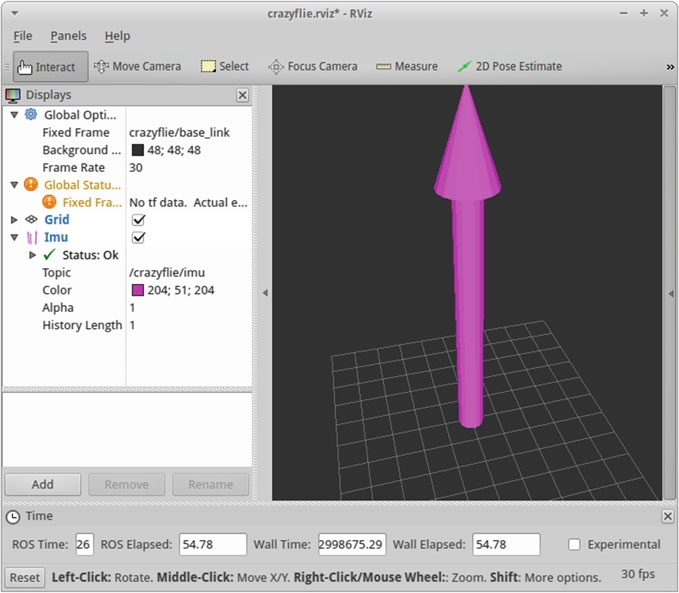
\includegraphics[scale=0.5]{rviz.png}
 \caption{rviz windows with IMU readings}
 \label{figure:rviz_demo}
\end{figure}

The rviz window displays data received from the CrazyFlie IMU as seen in Figure \ref{figure:rviz_demo}.If the drone is tilted the arrow should be pointing in the relevant direction.

\subsection{Obtaining the position of the drone}
Position estimate is required to make the drone fly autonomously and a method is needed to make the \texttt{crazyflie\_ros} stack aware of the position reported by the Optitrack system. The Optitrack server transmits the position of individual and a Linux PC is connected to the server with an ethernet cable. The basic functionality is shown in Figure \ref{figure:diagram_crazyflie_system} below.

\label{section:ws3}
\begin{figure}[H]
\centering
 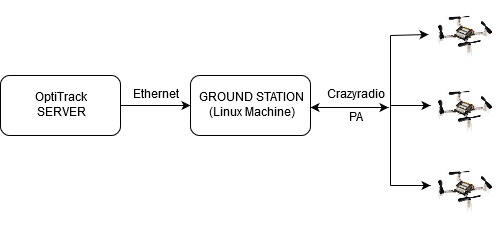
\includegraphics[scale=0.5]{crazyflie_system.png}
 \caption{Diagram of the crazyflie system}
 \label{figure:diagram_crazyflie_system}
\end{figure}

The way ROS nodes communicate is by publishing and subscribing to topics. This means that a special ROS node is needed that publishes location data from the OptiTrack server and the ROS node controlling the crazyflie needs to subscribe to it.\\
Optitrack is capable of sending data by using VRPN\cite{web_vrpn_wiki} so the first approach is to install an existing vrpn client and connect it directly to the Optitrack server.\\

\noindent The following instruction assume that two crazyflie drones are being tracked by Optitrack, named cf1 and cf2 respectvely. As a first step vrpn client is installed:

\begin{mdframed}[backgroundcolor=light-gray, linecolor=light-gray]
\texttt{\$ sudo apt-get install ros-kinetic-vrpn-client-ros}
\end{mdframed}

\noindent A custom \texttt{vrpn.launch} file is created with the specification of the Optitrack server. The file must be located at the path \texttt{vrpn-client-ros} is installed so the directory is changed as such:
\begin{mdframed}[backgroundcolor=light-gray, linecolor=light-gray]
\texttt{\$ roscd vrpn\_client\_ros\/launch\/}
\end{mdframed}

\noindent Next a new file is created e.g. by using \texttt{nano}:
\begin{mdframed}[backgroundcolor=light-gray, linecolor=light-gray]
\texttt{\$ nano vrpn.launch}
\end{mdframed}

\noindent and the following contents are added to the file:

\begin{minted}[breaklines, linenos,frame=single]{xml}
<launch>

  <arg name="server" default="192.168.0.100"/>

  <node pkg="vrpn_client_ros" type="vrpn_client_node" name="vrpn_client_node" output="screen">
    <rosparam subst_value="true">
      server: $(arg server)
      port: 3883

      frame_id: world
      broadcast_tf: true

      # Must either specify refresh frequency > 0.0, or a list of trackers to create
      refresh_tracker_frequency: 1.0
      #trackers:
      #- FirstTracker
      #- SecondTracker
    </rosparam>
  </node>
</launch>
\end{minted}

\noindent where if \textit{refresh\_tracker\_frequency} is specified the ROS node receives the position of all tracked Optitrack objects. Specifying objects by name returns only their position.\\
\noindent Once the created file is saved, the vrpn client is run by using the launch file above:

\begin{mdframed}[backgroundcolor=light-gray, linecolor=light-gray]
\texttt{\$ roslaunch vrpn\_client\_ros vrpn.launch}
\end{mdframed}

\noindent The following command is run in a new terminal:
\begin{mdframed}[backgroundcolor=light-gray, linecolor=light-gray]
\texttt{\$ rosrun tf view\_frames}
\end{mdframed}
\noindent This last command generates a \texttt{frames.pdf} file describing the transmitted frames as in the Figure \ref{figure:ros_vrpn_frames} below.

\begin{figure}[H]
\centering
 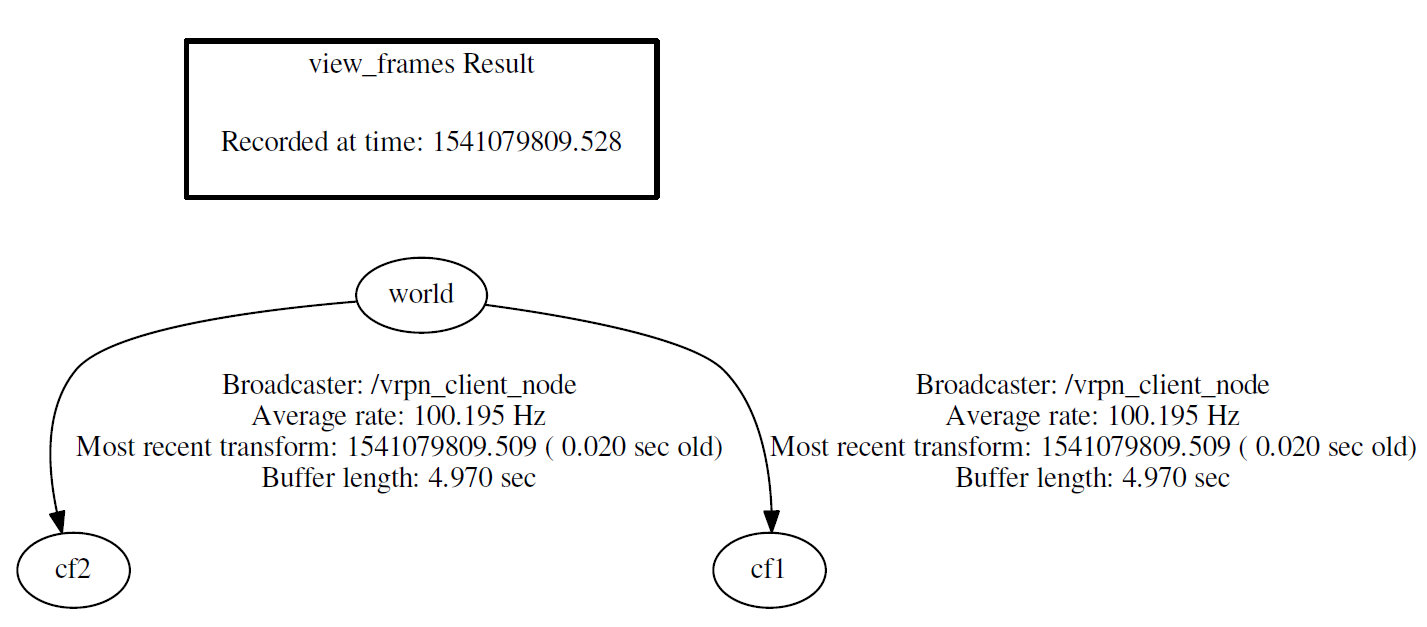
\includegraphics[scale=0.5]{frames.png}
 \caption{The result of running \texttt{view\_frames} using the VRPN node. Two tracked crazyflies named cf1 and cf2 can be observed}
 \label{figure:ros_vrpn_frames}
\end{figure}

\noindent To check what data is being transmitted position data the \texttt{tf\_echo} command can be used as such:

\begin{mdframed}[backgroundcolor=light-gray, linecolor=light-gray]
\begin{verbatim}
$ rosrun tf tf_echo /world /crazyflie1
At time 1542987286.924
- Translation: [1.711, 0.439, 2.254]
- Rotation: in Quaternion [-0.011, 0.675, -0.019, 0.738]
            in RPY (radian) [-0.436, 1.473, -0.447]
            in RPY (degree) [-24.999, 84.392, -25.621]
\end{verbatim}
\end{mdframed}

\noindent where \texttt{crazyflie1} is the name of the Rigid Body in Optitrack. The data displayed by \texttt{tf\_echo} shows the translation (in metres) and orientation (in Quaternions and Euler angles) of the \textit{crazyflie1} drone frame relative to the static \textit{world} frame.\\

\noindent The \textit{Translation} part of the frame reports the $x, y, z$ coordinates as reported by Optitrack and do not translate well to the SmartCity representation (see Table \ref{table:smartcity-to-optitrack}). \textit{Rotation} shows the attitude of the drone in Quaternions and $roll, pitch, yaw$ Euler angles. These values are also wrong since Optitrack reports these values in the $pitch, yaw, roll$ order while the vrpn client reads them in the $roll, pitch, yaw$ order.

\noindent The vrpn client also publishes ROS Pose messages which allows viewing the drones in tools such as \texttt{rviz}. Separate topics are created for each tracked crazyflie as seen in the result of \texttt{rostopic list} below:
\begin{mdframed}[backgroundcolor=light-gray, linecolor=light-gray]
\begin{verbatim}
$ rostopic list
/rosout
/rosout_agg
/tf
/vrpn_client_node/crazyflie1/pose
/vrpn_client_node/crazyflie2/pose
\end{verbatim}
\end{mdframed}.

\noindent Using \texttt{rviz} to view the published drone poses it can be quickly observed that if drones are moved, by example upwards, the rviz object will not move in the expected up direction but instead move towards the expected x or y direction. This makes using the vrpn system client unreliable and extra steps that account for correcting the translation and rotation axes need to be taken. This leads to the section which investigates the use of a custom Optitrack server which correctly translates Optitrack position to the SmartCity layout.


\subsection{Using a custom Optitrack server}
The Optitrack custom server named \textit{OptitrackGPS} has been written by the SmartCity team and the authors of this project have been granted access to their private repository. \textit{OptitrackGPS} reports object position and rotation correctly in the SmartCity layout and it requires a special client to connect to it.\\

\noindent The client used to connect to the server is also written by the SmartCity team. Its intended use is to run on the onboard computer of every tracked device. However for this project the client runs on a single PC and it transmits position data to all connected crazyflies. This is deemed a more convenient approach in using the crazyflie ros stack rather than modifying the crazyflie firmware to allow communication via Bluetooth or the CrazyRadio protocol (the only wireless communication metgods that the crazyflie supports).\\

\noindent A separate ROS package is created containing the default SmartCity GPS code, modified to function as a ROS node, publishing location data to the \texttt{server\_messages} topic. The amended code can be seen in the listing below:

\noindent First the ROS package is created with the required dependencies:
\begin{mdframed}[backgroundcolor=light-gray, linecolor=light-gray]
\begin{verbatim}
$ cd ~/crazyflie_ws/src
$ catkin_create_pkg servicelayer_gps_ros std_msgs roscpp
\end{verbatim}
\end{mdframed}

\noindent In the same directory all the required header files for the SmartCity GPS.cpp are added to the \texttt{include/servicelayer\_gps\_ros/} folder. The GPS.cpp file itself is copied to the \texttt{servicelayer\_gps\_ros/src} folder and modified as such:

\begin{code}
\begin{minted}[breaklines, linenos,frame=single]{cpp}
// SmartCity includes
#include "ros/ros.h"
#include "std_msgs/String.h"
#include <sstream>

// GPS.cpp code

DataStorage_t Data;
int main(int argc, char **argv)
{
  ros::init(argc, argv, "servicelayer_gps");
  ros::NodeHandle n;
  
  ros::Publisher chatter_pub = n.advertise<std_msgs::String>("/server_data/", 1000);
  Data.vehicleID << (uint8_t)(111);

  GPS * gps = new GPS(&Data);
  GPS_Data pose;

  ros::Rate loop_rate(100);

  while (ros::ok())
  {
    std_msgs::String msg;
    pose = Data.GPS.pop();

    std::stringstream ss;
    ss << "X: " << pose.x << " Y: " << pose.y << " Z: " << pose.z << " YAW: " << pose.yaw;
    msg.data = ss.str();

    chatter_pub.publish(msg);

    ros::spinOnce();

    loop_rate.sleep();
  }
  return 0;
}
\end{minted}
\caption{The source code for the servicelayer\_gps node. Made to publish the position of a specific drone as a string.\\}
\label{listing:servicelayer_v1}
\end{code}

\noindent Particular code lines from the above listing are explained below:

\begin{minted}[breaklines, frame=single]{cpp}
  ros::Publisher chatter_pub = n.advertise<std_msgs::String>("/server_data/", 1000);
\end{minted}
\noindent Make the ROS node publish text data to a topic named \textit{/server\_data}

\begin{minted}[breaklines, frame=single]{cpp}
  Data.vehicleID << (uint8_t)(111);
\end{minted}
\noindent The OptitrackGPS server requires the client to specify the id of the tracked object and it only tracks objects that respect the "RigidBody x" naming scheme, where \textit{x} is an unsigned integer in the 0-255 range. Therefore the previously drones previously named \textit{crazyflie1} and \textit{crazyflie2} are renamed to \textit{RigidBody 111} and \textit{RigidBody 222} respectively. The integer part is the one that needs to be passed to the server and in this instance the connection to \textit{RigidBody 111} is tested.

\begin{minted}[breaklines, frame=single]{cpp}
  GPS * gps = new GPS(&Data);
\end{minted}
\noindent Create a servicelayer GPS object and use \textit{Data} to store information.

\begin{minted}[breaklines, frame=single]{cpp}
  ros::Rate loop_rate(100);
  //.....
  loop_rate.sleep();
\end{minted}
\noindent Run the loop at a frequency of 100 Hz.

\begin{minted}[breaklines, frame=single]{cpp}
  pose = Data.GPS.pop();
\end{minted}
\noindent Assign the last position data received from Optitrack($x,y,z, yaw$) to the \textit{pose} variable

\noindent After this the \texttt{CMakeLists.txt} file must be modified in order for the newly created package to be built.

\begin{mdframed}[backgroundcolor=light-gray, linecolor=light-gray]
\begin{verbatim}
$ cd ~/crazyflie_ws/src/servicelayer_gps_ros
$ nano CMakeLists.txt
\end{verbatim}
\end{mdframed}

\noindent , where under the \texttt{\#\# Build \#\#} section the \textit{include\_directories()} function is modified as follows:
\begin{minted}[breaklines, frame=single]{cmake}
include_directories(
  ${catkin_INCLUDE_DIRS}
  include/${PROJECT_NAME}
)
\end{minted}
\noindent and at the end of the file the following lines are added:
\begin{minted}[breaklines, frame=single]{cmake}
set (CMAKE_CXX_STANDARD 11)
add_executable(GPS src/GPS.cpp)
target_link_libraries(GPS ${catkin_LIBRARIES})
\end{minted}

\noindent As the last step the package is compiled and built:
\begin{mdframed}[backgroundcolor=light-gray, linecolor=light-gray]
\begin{verbatim}
$ cd ~/crazyflie_ws/
$ catkin_make
\end{verbatim}
\end{mdframed}

Before the server is tested the crazyflies are put in the same place as shown in Figure \ref{figure:smart_city_layout} and it is ensured that the PC is connected to the same network as the Optitrack server via an ethernet cable. Then the newly create package is run:
\begin{mdframed}[backgroundcolor=light-gray, linecolor=light-gray]
\begin{verbatim}
$ rosrun servicelayer_gps_ros GPS
\end{verbatim}
\end{mdframed}
\noindent , and in a separate \texttt{rostopic echo} is run to check the data published by the gps node:
\begin{mdframed}[backgroundcolor=light-gray, linecolor=light-gray]
\begin{verbatim}
$ rostopic echo /server_data
---
data: "X: 2.254 Y: 1.711 Z: 0.439 YAW: 84.392"
---
\end{verbatim}
\end{mdframed}
\noindent Here it can be verified that the connection to the server works and the reported $x, y, z$ and $yaw$ values are compatible with the SmartCity layout (see Table \ref{table:smartcity-to-optitrack}).\\

\noindent In the next section the gps node is adapted to publish data compatible with the crazyflie ros stack \texttt{crazyflie\_controller} and perform the first autonomous test flights.